% Lecture Template for ME3001-001-Tristan Hill - Spring 2017
% 
% Mechanical Engineering Analysis with MATLAB
%
% Roots of Non- Linear Equations - Lecture 3
% MATLAB review

% Document settings
\documentclass[11pt]{article}
\usepackage[margin=1in]{geometry}
\usepackage[pdftex]{graphicx}
\usepackage{multirow}
\usepackage{setspace}
\usepackage{hyperref}
\usepackage{color,soul}
\usepackage{fancyvrb}
\usepackage{framed}
\usepackage{wasysym}
\usepackage{multicol}

\pagestyle{plain}
\setlength\parindent{0pt}
\hypersetup{
    bookmarks=true,         % show bookmarks bar?
    unicode=false,          % non-Latin characters in Acrobat’s bookmarks
    pdftoolbar=true,        % show Acrobat’s toolbar?
    pdfmenubar=true,        % show Acrobat’s menu?
    pdffitwindow=false,     % window fit to page when opened
    pdfstartview={FitH},    % fits the width of the page to the window
    pdftitle={My title},    % title
    pdfauthor={Author},     % author
    pdfsubject={Subject},   % subject of the document
    pdfcreator={Creator},   % creator of the document
    pdfproducer={Producer}, % producer of the document
    pdfkeywords={keyword1} {key2} {key3}, % list of keywords
    pdfnewwindow=true,      % links in new window
    colorlinks=true,       % false: boxed links; true: colored links
    linkcolor=red,          % color of internal links (change box color with linkbordercolor)
    citecolor=green,        % color of links to bibliography
    filecolor=magenta,      % color of file links
    urlcolor=blue           % color of external links
}

% assignment number 
\newcommand{\NUM}{2} 
\newcommand{\VSpaceSize}{2mm} 
\newcommand{\HSpaceSize}{2mm} 

\definecolor{mygray}{rgb}{.6, .6, .6}

\setulcolor{red} 
\setstcolor{green} 
\sethlcolor{mygray} 

\begin{document}

\textbf{ \LARGE ME 3001 Lecture, Roots of Non-Linear Equations} \\\\
\textbf{ \LARGE A Brief Overview of Optimization} \\

\begin{itemize}

	\item  \textbf{\LARGE First, A review the Bisection Method}
		
		\LARGE
		\begin{itemize}
			\item The algorithm \vspace{80mm}			
			\item The code
		\end{itemize}	
		\newpage

	\item \textbf{\LARGE What is Optimization ?}
		\begin{itemize}
			\item Find Local Minima and Maxima \vspace{80mm}	
			\item Constraints	
		\end{itemize}
		\newpage
		
	\item \textbf{\LARGE Root finding and Optimzation?}
		\begin{itemize}
			\item Using the derivative \vspace{80mm}	
			\item Constraints	
		\end{itemize}
		\newpage

	\item \textbf{\LARGE Optimzation Techniques}\\\\
		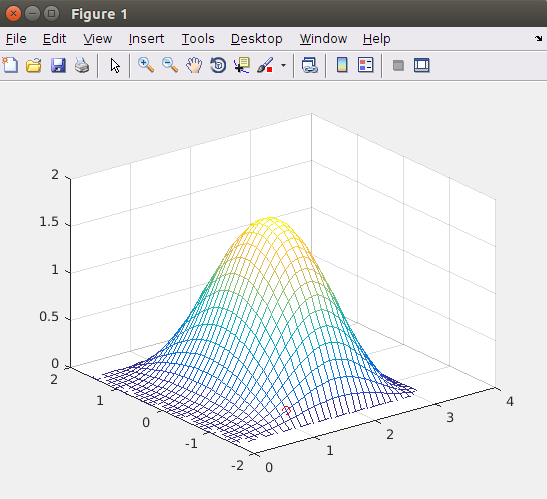
\includegraphics[scale=1]{lecture4_fig1.png}
		\begin{itemize}
			\item Brute Force \vspace{30mm}
			\item Steepest Accent	
		\end{itemize}
		\newpage


\newpage 

	\item \textbf{ \LARGE REMINDER - Homework 1 is due (11:59 PM) } \\
	
	\item \textbf{ \LARGE REMINDER - See instructions for submitting hw 1 - please resubmit} \\	
	 
	\item \textbf{ \LARGE REMINDER - MATLAB script from today's lecture will be posted on ilearn. } \\
		
	\item \textbf{ \LARGE REMINDER - A simpler version of the code from yesterday's lecture is posted on ilearn. } \\	

\end{itemize}


	

\end{document}



